\epigraph{You're the chosen one, Cuckoo.}{Adriaan}

\textbf{TOEKOMSTIGE TIJD}

For the Proof of Concept (PoC), Cuckoo \cite{cuckoo} will be used. Cuckoo is a malware analysis system that runs malware in a virtual environment, tracks its behavior and reports these results to the user.\\

Cuckoo was choosen because it already implements a great deal of the prerequisites of the algorithm, discussed in \todo{add ref}. Cuckoo, through Cuckoomon \cite{cuckoomon}, provides a series of hooks which monitors calls between the browser and the operating system. This allows us to monitor the extra information from section \ref{algo2}. 

These hooks, conveniently, also monitor the network calls made by the browser. Although only Internet Explorer is supported by Cuckoo, due to the scope of the project, this is not a problem.

\subsubsection{Prerequisites and changes}

Internet Explorer uses Windows' ``Secure Channel'' or ``Schannel'' \cite{schannel} to encrypt HTTP requests and decrypt HTTP responses. This will allow us to monitor traffic on the operating system level without any need for a proxy to decrypt the traffic.

As already explained, Cuckoo uses Cuckoomon, which uses hooks to monitor calls, to keep track of the browser activity. Besides adding a few new hooks and deleting a few irrelevant hooks for drive-by downloads, nothing major has to be changed to Cuckoomon.\todo{Uitleggen welke hooks precies?}

The current development version, \texttt{1.2-dev},  only accepts one URL at a time. To allow for concurrently visiting multiple websites in one sandbox environment, Cuckoo has to be extended.

\subsubsection{The Setup}

To test the algorithm, we will use the adapted Cuckoo with Virtualbox as the sandbox environment. As the virtual machine's operating system, we will use Windows 7 as this is still the operating system which is most targeted by malware. As the browser, we will use Internet Explorer 8 to actually allow the malware to successfully perform the drive-by download.

The virtual machine will be provisioned with the Top 20 of visited websites in the Netherlands, according to Alexa \cite{http://www.alexa.com/topsites/countries/NL}, and with current malware floating on the internet.\todo{Mss toch niet zeggen?}

The structure of the graph will be tree-like, as suggested in \todo{ref naar algo}. Figure \ref{fig:alg_tree}.

Figure \ref{fig:alg_tree} also shows a website with a drive-by download. In the top left, one can see process spawns (red vertices) in an unusual place.\todo{beter uitleggen}

\begin{figure}[h]
    \centering
    \centerline{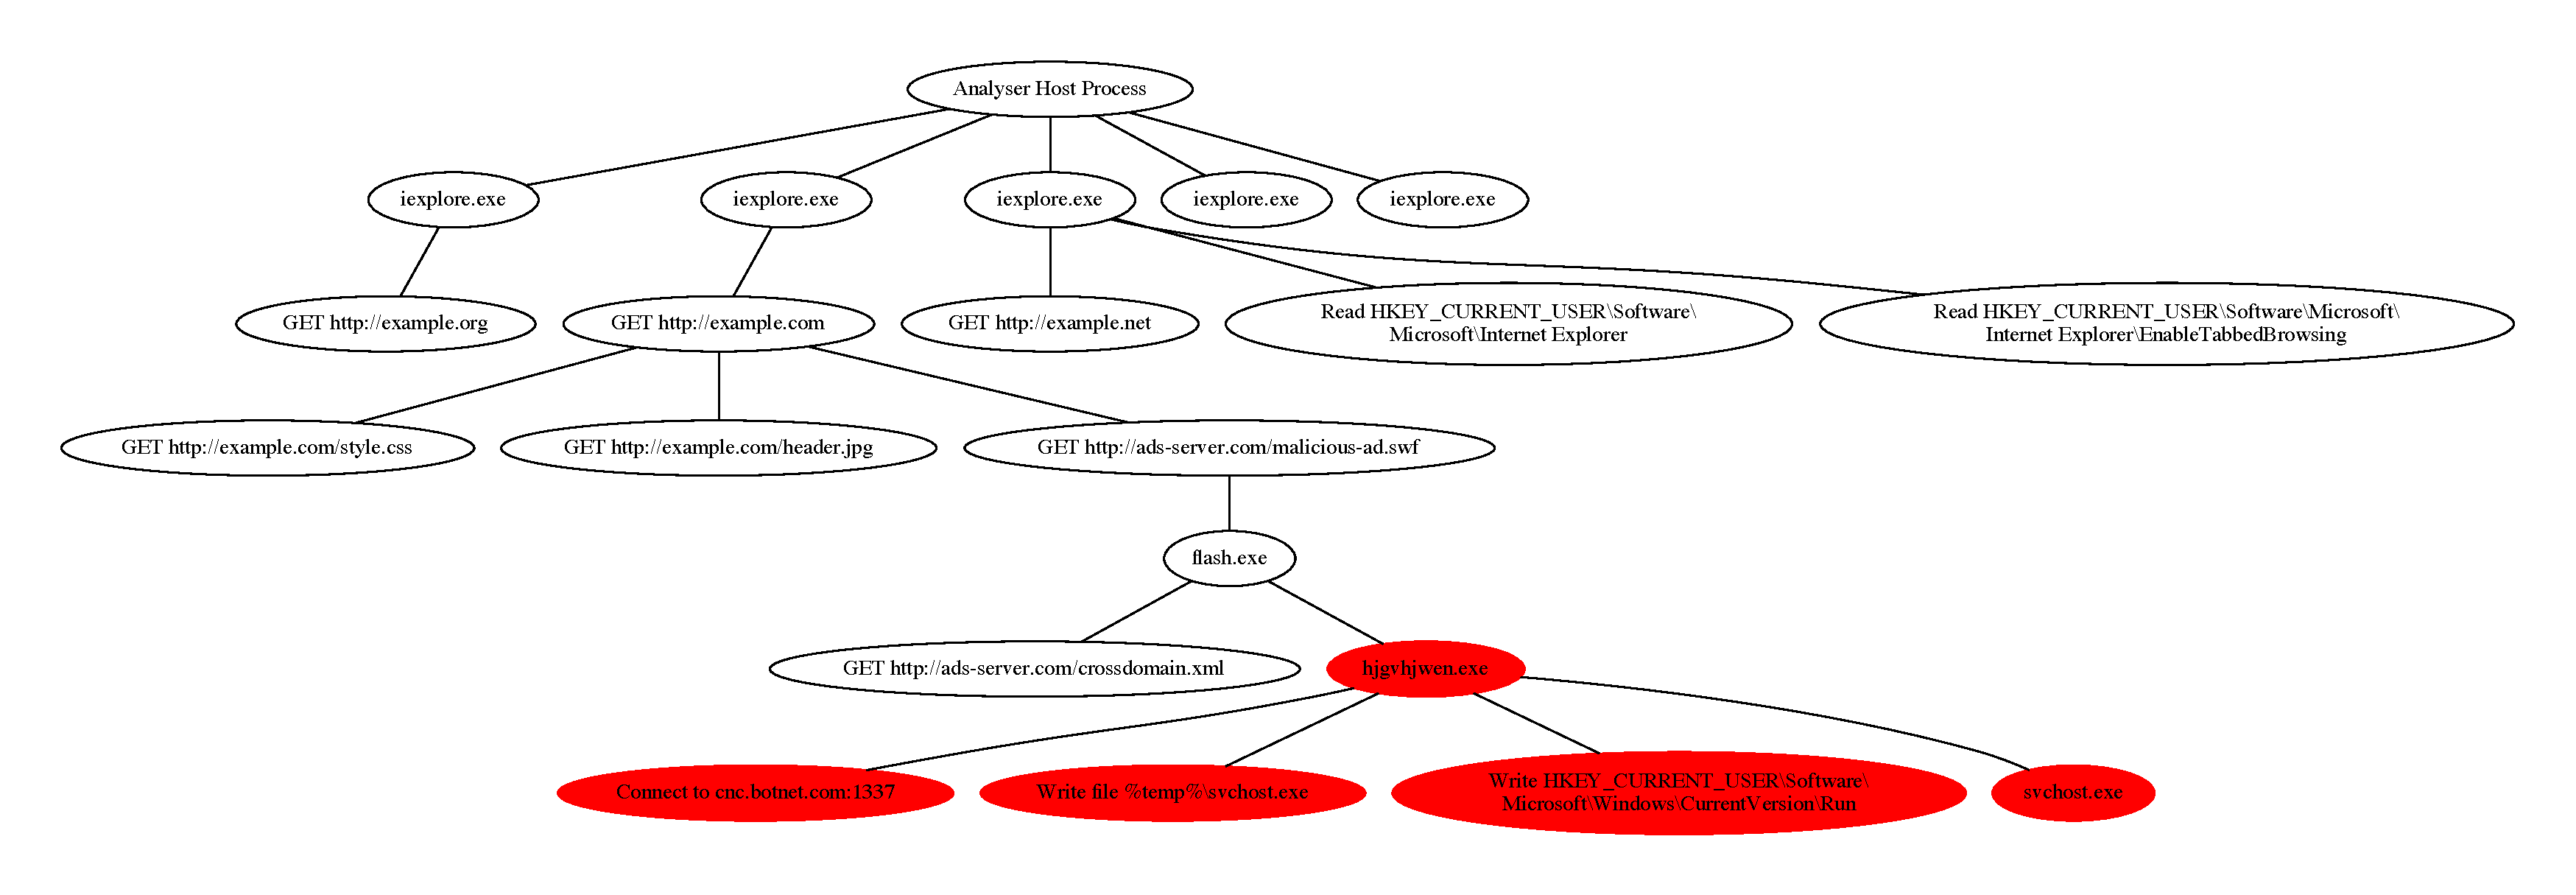
\includegraphics[width=19cm]{Images/alg_tree}}
    \caption{An example of the graph}
    \label{fig:graph}
\end{figure}

